% LaTeX Generic essay template
% Copyright (C) 2017  Shen Zhou Hong <shen@hong.io>
%
% This program is free software: you can redistribute it and/or modify
% it under the terms of the GNU General Public License as published by
% the Free Software Foundation, either version 3 of the License, or
% (at your option) any later version.
%
% This program is distributed in the hope that it will be useful,
% but WITHOUT ANY WARRANTY; without even the implied warranty of
% MERCHANTABILITY or FITNESS FOR A PARTICULAR PURPOSE.  See the
% GNU General Public License for more details.
%
% You should have received a copy of the GNU General Public License
% along with this program.  If not, see <https://www.gnu.org/licenses/>.

% For more information on documentclass configuration, see:
% https://texblog.org/2013/02/13/latex-documentclass-options-illustrated/#formula
\documentclass[
  12pt,       % 10pt, 11pt, 12pt
  a4paper,    % a4paper, letterpaper, a5paper, b5paper, executivepaper, legalpaper
  final,      % draft
  onecolumn,  % twocolumn
  oneside,    % twoside
  notitlepage % titlepage
]{article}

% Included documents in the preamble. Caution: Their order is important!
\usepackage[l2tabu, orthodox]{nag}
\usepackage[factor=2000]{microtype}
\usepackage{setspace}               % Used to change line and paragraph spacing
\usepackage{csquotes}               \MakeOuterQuote{"}
\usepackage[T1]{fontenc}            % Supports international fonts
\usepackage[osf]{libertine}         % Beautiful libertine font
\usepackage[parfill]{parskip}       % For empty lines between paragraphs
\usepackage{fancyhdr}               % For fancy headings
\usepackage{hyperref}               % So citations can be links
\usepackage{titling}                % In order to make the title higher on page
\usepackage{float}                  % Tell a float to stay HERE! [H]

% Optional LaTeX packages for additional functionality
% \usepackage[noframe]{showframe}     % Debug option to show margin frames.
\usepackage{graphicx}               % Required for embedding images
\usepackage{booktabs}               % For prettier tables
% \usepackage{geometry}             % Sets more "reasonable" margin-sizes
% \usepackage{tikz}                 % Used for graphical illustrations.
% \usetikzlibrary{calc,intersections,through,backgrounds}
\usepackage{amsmath}              % Needed for most math things.
\usepackage{amssymb}
\usepackage{mathtools}
% \usepackage{gensymb}              % For degree symbol \degree
\usepackage{multicol}               % For fancy tables that look nice.
\usepackage{mathtools}
% \usepackage{svg}                    % Allows embedding svg \includesvg{path}
\usepackage{siunitx}


\usepackage{makecell}
\setcellgapes{4pt}
% The biblatex package should go last!
% FYI: the biblatex package is used to generate a bibliography. However, unless
% intense citation management (e.g. 5+ sources) is used, biblatex should not
% be loaded, as it slows down the document compilation process by almost 2X.
% In order to enable it, see sections/endpage.tex and essay-name.tex's preamble
%
% \usepackage[style=mla, backend=biber]{biblatex} % Nice MLA bibliography

% Settings used by \usepackage{microtype}
% These custom hyphenation rules are used to discourage excessive hyphenation
\pretolerance=5000
\tolerance=9000
\emergencystretch=0pt
\righthyphenmin=4
\lefthyphenmin=4
\microtypecontext{spacing=nonfrench}

% Settings used by \usepackage{setspace}
% These commands are used to change the line-spacing of the text.
% Use \linespread{1.25} for custom line spacing.
% See documentation at https://tex.stackexchange.com/questions/65849/
% \doublespacing  for double-spacing
\onehalfspacing % for 1.5 spacing

% Settings used by \usepackage[parfill]{parskip}
\setlength{\parindent}{3em} % Paragraph indentation. Set to 0em to disable.

% Settings used by \usepackage{titling}
% The following command is used to "hang" the default LaTeX title from the top
% of the page (e.g. like a painting frame). The default LaTeX title sits a bit
% too low, so the following command sets it higher.
\setlength{\droptitle}{-4em}   % This is your set screw

% \addbibresource{citations.bib} Biblatex. See includes/formatting.tex

% Document Metadata
\title{
  \textbf{\textsc{The Math Behind Paper}} \\ Investigating Geometric Sequences Behind the \mbox{ISO 216} Series-A Paper Format
}
\author{
  By Shen Zhou Hong \and Goldsmiths, University of London
}
\date{\today}

% Document Begins
\begin{document}
\maketitle
% \tableofcontents Optional table-of-contents
% \clearpage clears page on table of contents so content starts on new page.

% Includes content body. If the essay is very long, it might make sense to split
% the content across multiple .tex files, and include them all here, e.g.
% \input{sections/preamble.tex}

\begin{figure}[H]
  \centering
  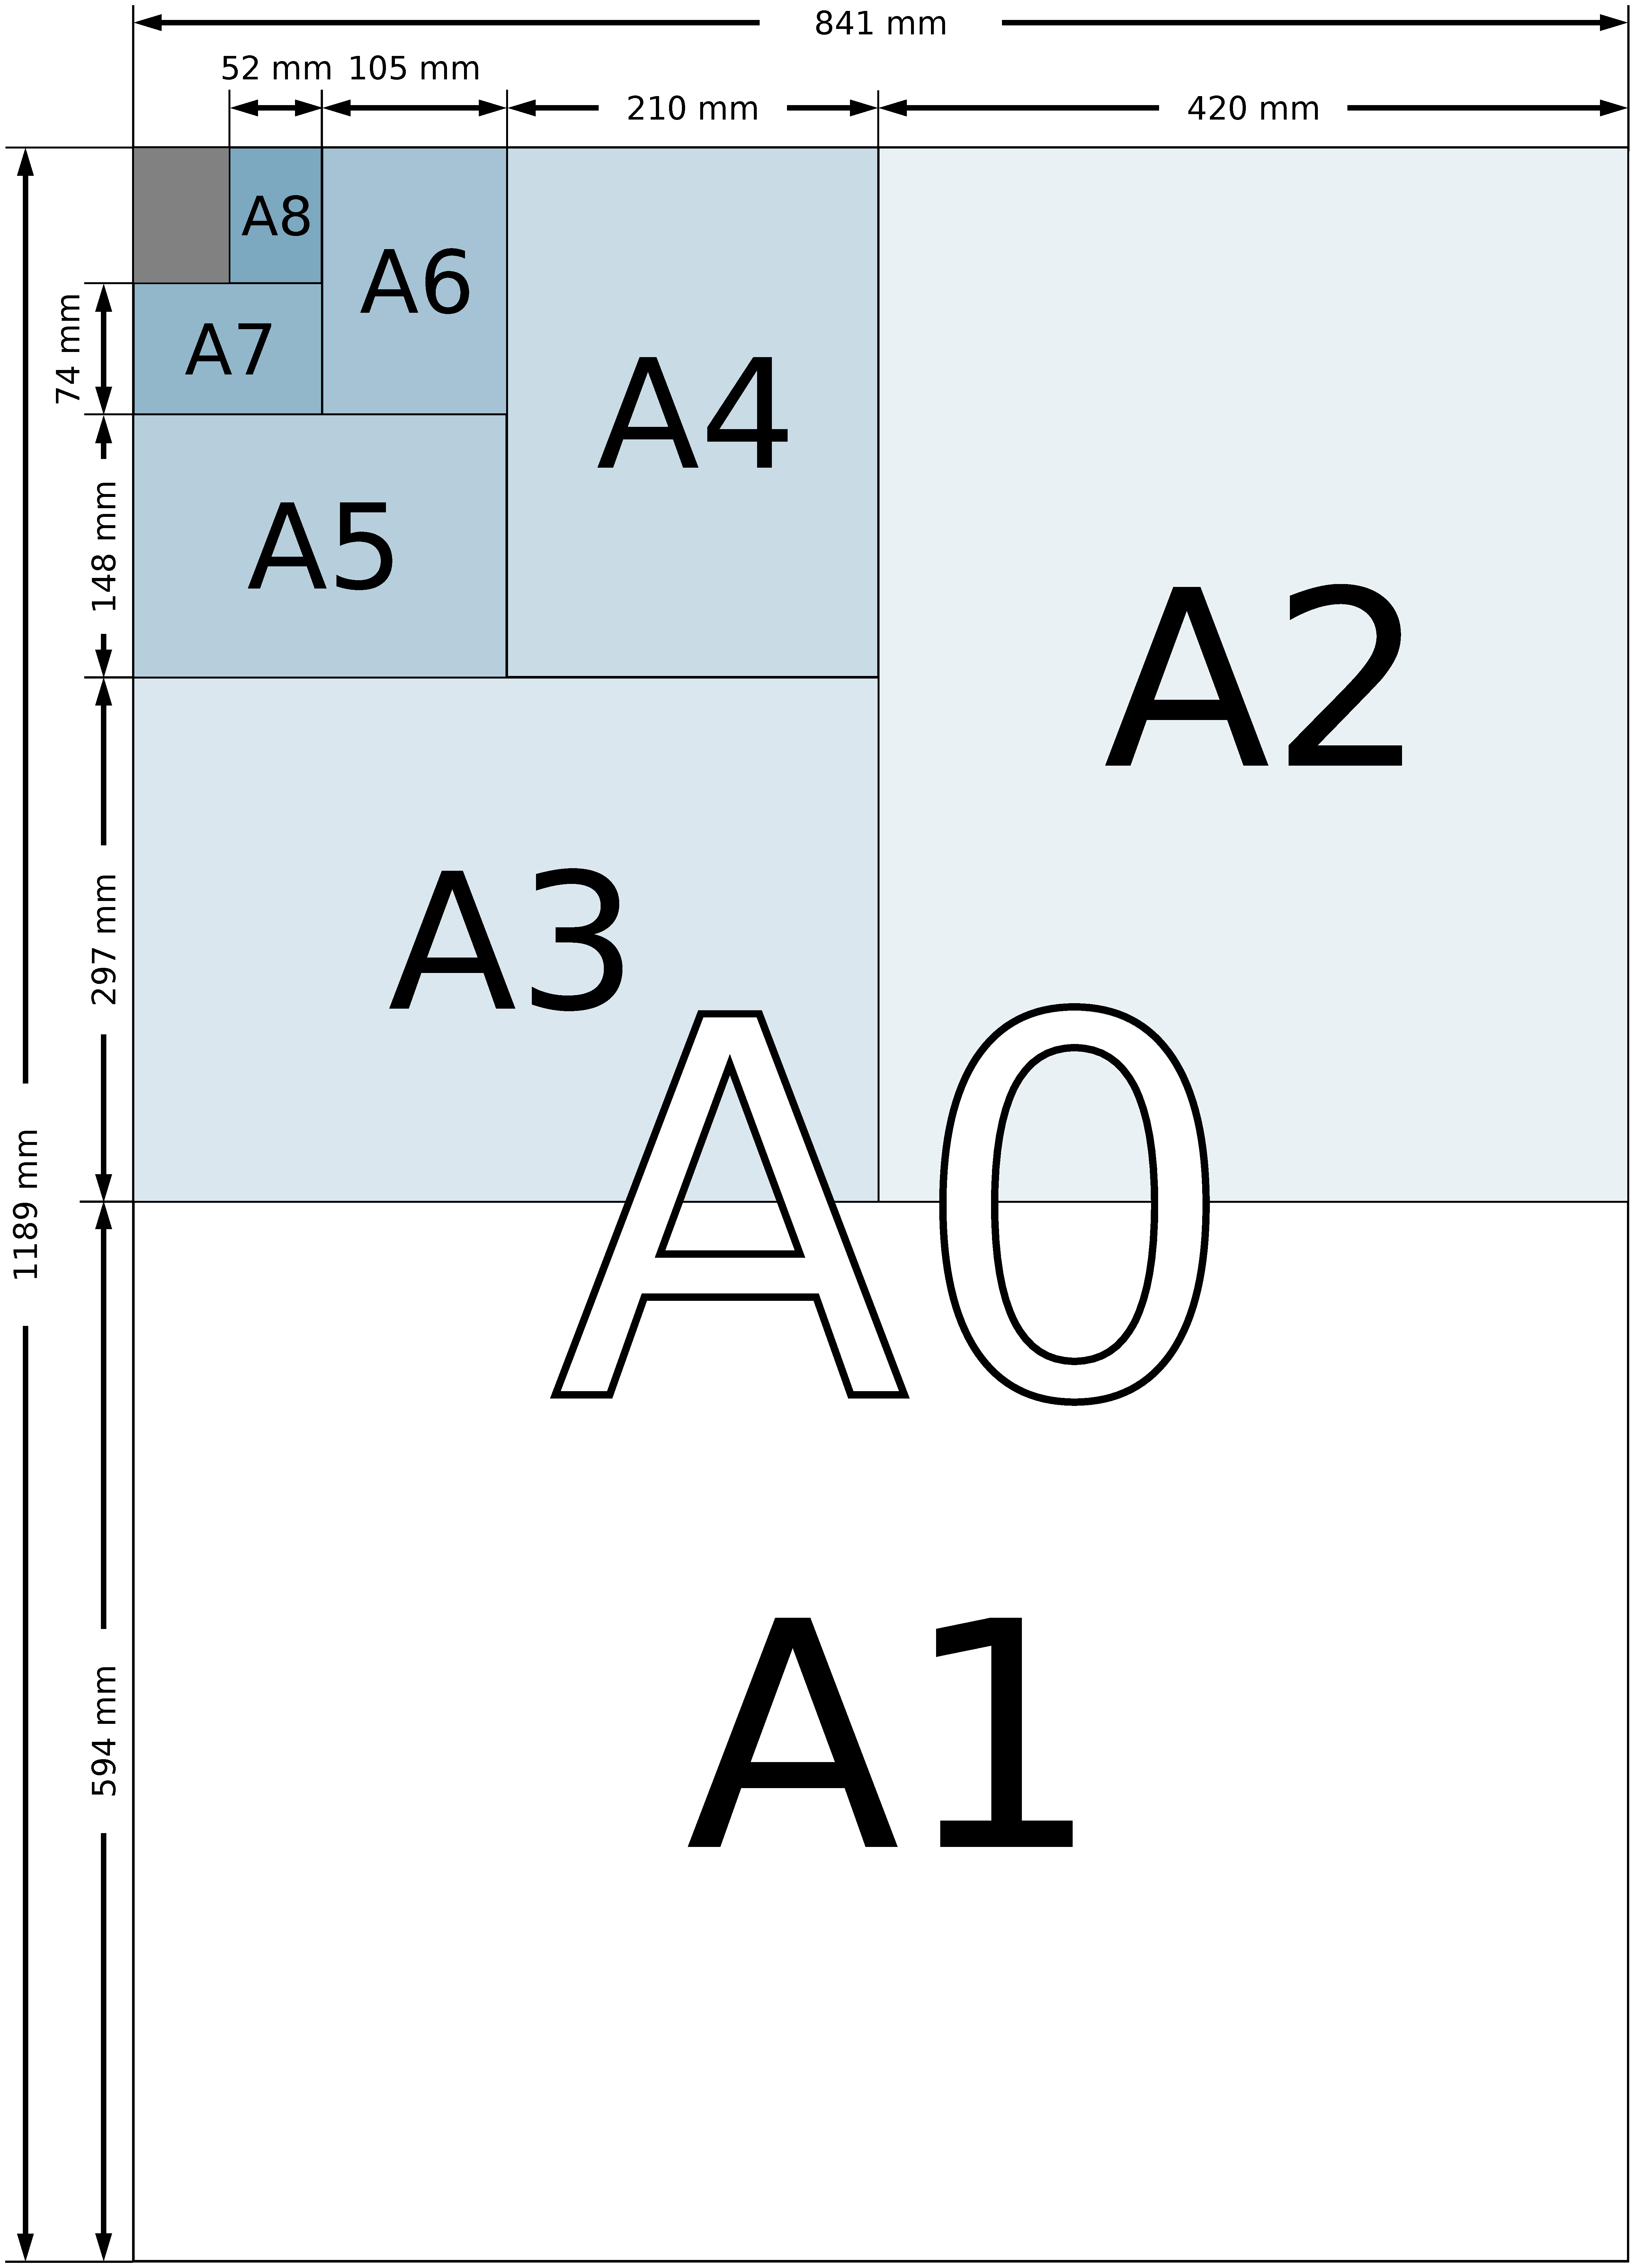
\includegraphics[angle=270,origin=c,width=0.8\textwidth]{includes/A-paper-eps}
\end{figure}

\section*{Introduction}
Understanding the properties of arithmetic and geometric sequences are essential for quantifying the world, and for computing in general. In this paper, I will investigate the different sizes of ISO 216 standard A-series paper, and quantify their properties using my knowledge of sequences.

\section*{The Properties of ISO 216 A-Series Paper}
Let us begin by quantifying the properties of ISO 216 A-series paper (henceforth referred to as A-paper). It is given that the largest A-paper size, $A_{0}$, has a total area of \SI{1}{\metre\squared}. Likewise, we know that each successive smaller paper is the previous paper folded in half.

\subsection*{Formalising the Area}
We can formalise this property as the following geometric sequence:

\begin{align*}
  a_{n} &= a \times r^{n - 1} \\
  A_{n} &= A \times \left(\frac{1}{2}\right)^{n -1} \\
        &= 2^{-n}
\end{align*}

\noindent
By plugging in the the numbers, it is trivial to generate a table of area for each successive A-series paper:

\begin{table}[h]
  \centering\makegapedcells
    \begin{tabular}{@{}lcl@{}}
    \toprule
    $n$ & Area (fractional \si{\meter\squared}) & Area (decimal \si{\meter\squared}) \\ \midrule
    $0$ & $1$               & $1$              \\
    $1$ & $\frac{1}{2}$     & $0.5$            \\
    $2$ & $\frac{1}{4}$     & $0.25$           \\
    $3$ & $\frac{1}{8}$     & $0.125$          \\
    $4$ & $\frac{1}{16}$    & $0.0625$         \\
    $5$ & $\frac{1}{32}$    & $0.03125$        \\
    $6$ & $\frac{1}{64}$    & $0.015625$       \\ \bottomrule
  \end{tabular}
  \caption{List of A-series paper areas for $0 \geq n \leq 6$}
  \label{tab:area}
\end{table}

\subsection*{Formalizing the Length and Width}
The geometric sequence behind the area of the A-series paper is trivial to discover, but what about the length and width of the paper for a given $n$ in $A_{n}$? Recall that every time an A-series paper is folded in half, we make the fold at the largest side (the length) of the paper:

\begin{align*}
  A_{n}     &= L_{n} \times W_{n} \\
  A_{n + 1} &= \frac{L_{n}}{2} \times W_{n}
\end{align*}

\noindent
Where essentially the new "length" of $A_{n + 1}$ is actually the width of the previous larger paper, namely $A_{n}$:

\begin{align*}
  L_{n + 1} &= W_{n} \\
  W_{n + 1} &= \frac{L_{n}}{2}
\end{align*}

\noindent
This relation is apparent even if we just list out the sequences:

\[
  \begin{array}{*{8}{l@{\ }}}
    L_{n} = & L_{0}, & \frac{L_0}{2}, & \frac{L_{0}}{2}, & \frac{L_{0}}{4}, & \frac{L_{0}}{4}, & \frac{L_{0}}{8}, & \frac{L_{0}}{8}, \\[\jot]
    W_{n} = & W_{0}, &         W_{0}, & \frac{W_{0}}{2}, & \frac{W_{0}}{2}, & \frac{W_{0}}{4}, & \frac{W_{0}}{4}, & \frac{W_{0}}{8},
  \end{array}
\]

\noindent
This property is an important one, because it allows us to discover the ratio, or \emph{aspect ratio} between the two sides of the paper. We must do this prior to the next section on the scaling factor, because without knowing the aspect ratio of the sides, there is no way for us to do proper scaling conversions. Hence, let $R_{n}$ be the aspect ratio of $A_{n}$

\begin{align*}
  R_{n}     &= \frac{L_{n}}{W_{n}} \\
  R_{n + 1} &= \frac{L_{n + 1}}{W_{n + 1}} \\
            &= \frac{W_{n}}{L_{n} \div 2} \\
            &= \frac{2W_{n}}{L_{n}} \\
            &= \frac{2}{L_{n} \div W_{n}}
\end{align*}

\noindent
Originally, I hoped that somehow the terms would cancel out and I would be able to have a numerical solution, but that didn't happen. However, not all was lost, because in the process of working out this math I came to another realisation. Now recall that we defined $R_{n}$ as $\frac{L_{n}}{W_{n}}$. Therefore:

\begin{align*}
  R_{n + 1} &= \frac{2}{L_{n} \div W_{n}} \\
            &= \frac{2}{R_{n}}
\end{align*}

\noindent
Do you recall how in the Lecture, we were told that one of the properties of the A-series paper, was how each time you fold it in half it preserves the proportions of the previous paper? This is a property that is unique to the ISO 216 paper, if you take a U.S. Letter paper and fold it in half, every time you fold it you end up with a slightly different rectangle. Now, there is only one way that this property can happen --- namely that the aspect ratio of each subsequent halve must be the same, e.g $R_{n} = R_{n + 1} = R_{n + 2}$ for $n \to \infty$ where the aspect ratio is $1:R_{n}$ Therefore:

\begin{align*}
  R_{n + 1} &= \frac{2}{R_{n}} = R_{n}
\end{align*}

\noindent
Now we have the simple numerical solution that I was looking for! We can find the value of $R_{n}$ simply by solving for it:

\begin{align*}
  R_{n} &= \frac{2}{R_{n}} \\
  R_{n} \times R_{n} &= 2 \\
  \left(R_{n}\right)^2 &= 2 \\
  R_{n} &= \sqrt{2}
\end{align*}

\noindent
Therefore, the aspect ratio of the ISO 216 A-series paper is $1:\sqrt{2}$. What does this mean? It means the ratio of the length to the width of the paper is that of $1:\sqrt{2}$, or expressed in Euclidean terms:\footnote{The Euclidean continuous proportion reads: "As $L_n$ is to $W_n$, in the manner of $1$ to $\sqrt{2}$".}

\begin{align*}
  L_n:W_n::1:\sqrt{2}
\end{align*}

\section*{Exact Algebraic Solutions to Lengths and Widths}
Now that we have laid the required groundwork in place, we can find the exact (and numerical approximations) solutions of the length and width for any arbitary $A_n$. This is done using the aspect ratio we discovered in the previous section.

\subsection*{Exact Algebraic Solution for $L_0$, $W_0$}
First, in order to create an expression that will find the $L_n$, $W_n$ for any $A_n$, we must find the $L_0$, $W_0$ of $A_0$. Given $A_0 = L_0 \times W_0$, and that $A_0 = 1$ (as by definition), a system of simulatneous equations of the 2nd order can be used to find the exact algebraic solutions to $L_0$, $W_0$:

\begin{align*}
  \begin{cases}
    L_0 \times W_0 &= 1 \\
    W_0 \times \sqrt{2} &= L_0
  \end{cases}
\end{align*}

\noindent
Note that $W_0 \times \sqrt{2} = L_0$ holds true due to the aspect ratio, as we discussed in the previous section. Hence, to solve for $W_0$, we substitute $L_0$ from the 2nd equation in the system:

\begin{align*}
  W_0 \times \sqrt{2} \times W_0 &= 1 \\
  \left(W_0\right)^2 \times \sqrt{2} &=1 \\
  \left(W_0\right)^2 &= \frac{1}{\sqrt{2}} \\
  W_0 &= \sqrt{\frac{1}{\sqrt{2}}} \\
  &= \left(2^{-\frac{1}{2}}\right)^{\frac{1}{2}} \\
  &= 2^{-\frac{1}{4}} \\
  &= \frac{1}{\sqrt[4]{2}}
\end{align*}

\noindent
With $W_0 = \frac{1}{\sqrt[4]{2}}$, finding the solution for $L_0$ is trivial:

\begin{align*}
  L_0 \times \frac{1}{\sqrt[4]{2}} &= 1 \\
  \frac{L_0}{1} \times \frac{1}{\sqrt[4]{2}} &= 1 \\
  \frac{\sqrt[4]{2}}{\sqrt[4]{2}} &= 1 \\
  L_0 &= \sqrt[4]{2}
\end{align*}

\noindent
Therefore, we now know the length and width for $A_0$, namely:

\begin{align*}
  L_0 &= \sqrt[4]{2} \\
  W_0 &= \frac{1}{\sqrt[4]{2}} \\
\end{align*}

\noindent
And to check if our work is correct, all we have to do is to multiply the length and the width together, and check if they give us an exact integer solution of $1\si{\meter\squared}$ for $A_0$'s area:

\begin{align*}
  L_0 \times W_0 &= 1 \\
  \sqrt[4]{2} \times \frac{1}{\sqrt[4]{2}} &= 1
\end{align*}

\subsection*{Generalised Exact Algebraic Solutions}
Now that we defined the length and width of $A_0$, creating an expression or function for the length and width of any subsequent $A_n$ is trivial. The solutions for $L_n$ and $W_n$ can be represented as geometric sequences of the form $a_{n} = a \times r^{n - 1}$, where $r = \frac{1}{\sqrt{2}}$ as each subsequent smaller paper size is effectively divided by the aspect ratio:

\begin{align*}
  L_n &= \sqrt[4]{2} \times \left(\frac{1}{\sqrt{2}}\right)^{n} \\
  W_n &= \frac{1}{\sqrt[4]{2}} \times \left(\frac{1}{\sqrt{2}}\right)^{n}
\end{align*}

\noindent
For the purpose of generating the required table of lengths and widths, we will represent those expressions as functions instead:

\begin{align*}
  L(n) &= \sqrt[4]{2} \times \left(\frac{1}{\sqrt{2}}\right)^{n} \\
  W(n) &= \frac{1}{\sqrt[4]{2}} \times \left(\frac{1}{\sqrt{2}}\right)^{n}
\end{align*}

\subsection*{Generated Table of Values for $A_0$ --- $A_4$}
Now that we have the functional form of the sequence notation, we can fulfill part 1 and 2 of the assignment by generating a table of the exact and approximative magnitudes of the length and width.

\noindent
Note that, in order to save space in the table, we will not use the pretty radical notation of the terms, but rather the more compact (and arguablly, less pretty) exponent notation:

\begin{align*}
  L_n = \sqrt[4]{2} \times \left(\frac{1}{\sqrt{2}}\right)^{n} &=
  2^{\frac{1}{4} - \frac{n}{2}}\\
  W_n = \frac{1}{\sqrt[4]{2}} \times \left(\frac{1}{\sqrt{2}}\right)^{n} &=
  2^{-\frac{1}{4} - \frac{n}{2}}\\
\end{align*}

\subsubsection*{Table of Exact Values\footnote{Note that the numbers following the $2$ are exponents, although the lack of space in the table can make them look like regular terms. For example, under the length column for $A_2$, the entry $2^{-\frac{3}{4}}$ reads "two to the power of negative three over four". Please don't confuse the small numbering with regular terms!}}
\begin{table}[H]
  \centering\makegapedcells
  \begin{tabular}{@{}llll@{}}
    \toprule
    Paper & Length (\si{\meter}) & Width (\si{\meter}) & Area (\si{\meter\squared}) \\ \midrule
    $A_0$ & $2^{\frac{1}{4}}$     & $2^{-\frac{1}{4}}$  & $1$     \\
    $A_1$ & $2^{-\frac{1}{4}}$    & $2^{-\frac{3}{4}}$  & $\frac{1}{2}$     \\
    $A_2$ & $2^{-\frac{3}{4}}$    & $2^{-\frac{5}{4}}$  & $\frac{1}{4}$     \\
    $A_3$ & $2^{-\frac{5}{4}}$    & $2^{-\frac{7}{4}}$  & $\frac{1}{8}$     \\
    $A_4$ & $2^{-\frac{7}{4}}$    & $2^{-\frac{9}{4}}$  & $\frac{1}{16}$    \\
    $A_n$ & $2^{\frac{1}{4} - \frac{n}{2}}$    & $2^{-\frac{1}{4} - \frac{n}{2}}$  & $\frac{1}{2^n}$    \\
    \bottomrule
  \end{tabular}
  \caption{Exact (algebraic) values for any given $A_n$}
  \label{tab:exact}
\end{table}

\noindent
Note that I have simplified the values to their simplest exponent form.

\subsubsection*{Table of Approximative Values}
\begin{table}[H]
  \centering\makegapedcells
  \begin{tabular}{@{}llll@{}}
    \toprule
    Paper & Length (\si{\meter}) & Width (\si{\meter}) & Area (\si{\meter\squared}) \\ \midrule
    $A_0$ & $1.1892$       & $0.8408$      & $1$      \\
    $A_1$ & $0.8408$       & $0.5946$      & $0.5$    \\
    $A_2$ & $0.5946$       & $0.4204$      & $0.25$   \\
    $A_3$ & $0.4204$       & $0.2973$      & $0.125$  \\
    $A_4$ & $0.2973$       & $0.2102$      & $0.0625$ \\ \bottomrule
  \end{tabular}
  \caption{Approximate (numerical) values for any given $A_n$}
  \label{tab:approx}
\end{table}

\noindent
Note that the figures are truncated to 3 decimal places.

\section*{Scaling Factor (e.g. Aspect Ratio) In Percentage}
As the final part of the assignment, we are tasked to calculate a "scaling factor" that allows us to easily convert between a given $A_n$ to $A_m$. A scaling factor is a number that we multiply the sides of the paper by, in order to reach a bigger or smaller sized paper. In order to do this, we use the aspect ratio $\sqrt{2}$, converted to a percentage. I will demonstrate this method as well as generate a table with percentage conversions as required.

\subsection*{Calculating Scaling Factor for arbitary $A_n$ to $A_m$}
Recall that the aspect ratio is calculated as $\sqrt{2}$. Therefore, to move "up" a paper size (e.g. from $A_n$ to $A_{n - 1}$), the given paper size is multiplied by $\sqrt{2}$. Likewise, to move "down" a paper size, the given paper size is divided by the same aspect ratio. Generalising towards a function for converting arbitary $A_n$ to $A_m$: 

\subsection*{Scaling Factor Table}
\begin{table}[h]
\centering\makegapedcells
\begin{tabular}{@{}lllllllll@{}}
\toprule
Size & A0     & A1    & A2    & A3    & A4    & A5    & A6      & A7      \\ \midrule
A0   & 100\%  & 71\%  & 50\%  & 35\%  & 25\%  & 18\%  & 12.50\% & 8.80\%  \\
A1   & 141\%  & 100\% & 71\%  & 50\%  & 35\%  & 25\%  & 18\%    & 12.50\% \\
A2   & 200\%  & 141\% & 100\% & 71\%  & 50\%  & 35\%  & 25\%    & 18\%    \\
A3   & 283\%  & 200\% & 141\% & 100\% & 71\%  & 50\%  & 35\%    & 25\%    \\
A4   & 400\%  & 283\% & 200\% & 141\% & 100\% & 71\%  & 50\%    & 35\%    \\
A5   & 566\%  & 400\% & 283\% & 200\% & 141\% & 100\% & 71\%    & 50\%    \\
A6   & 800\%  & 566\% & 400\% & 283\% & 200\% & 141\% & 100\%   & 71\%    \\
A7   & 1132\% & 800\% & 566\% & 400\% & 283\% & 200\% & 141\%   & 100\%   \\ \bottomrule
\end{tabular}
\caption{Scale Factors for Conversions between arbitrary $A_n$ to $A_m$. }
\label{tab:scale-factor}
\end{table}

\clearpage
% Uncomment for bibliography using biblatex (see includes/formatting.tex)
% \section*{Bibliography}
% Print every citation in citations.bib, even if unused by \autocite
% \nocite{*}
% \printbibliography[heading=none]

\section*{Research credit}
Special thanks to Giuseppe Stelluto for his demonstration of an alternative method for deriving the formula for the sequences $L_n$ and $W_n$. His approach was much more technically rigorous, but I felt that my approach was more accessible to those without a formal education in mathematics.

\noindent
Additional thanks to \href{https://www.papersizes.org}{papersizes.org} for supplying an CSV (comma seperated values) file with the scaling factors. Originally I was making the table by hand in LaTeX, but that literally took forever. With an premade CSV file, I was able to work much faster, and simply convert the CSV format to a \LaTeX\ table.

\section*{Image credit}
\href{https://en.wikipedia.org/wiki/File:A_size_illustration2.svg}{Cover page illustration is a diagram illustrating ISO 216 A-series paper sizes, sourced from Wikipedia under Creative Commons (CC BY-SA 3.0) license.}

\section*{Technical Notes}
This essay is typeset using \LaTeX, an Open Source document typesetting language
by Donald Knuth, and version-controlled via Git. The git repository containing notes, source code, and revision history is available upon request.

% Optional: Include github URL here

\noindent
This essay is written using the EssayTemplate, an open source \LaTeX\ essay
template designed for the Humanities by Shen Zhou Hong. It is available at:

https://github.com/ShenZhouHong/EssayTemplate

\vfill
\begin{center}
This \LaTeX\ essay is also available in Microsoft Word, OpenOffice, HTML, and \mbox{plain text} upon request.
\end{center}


\end{document}
